\documentclass[12pt,a4paper]{article}

% Pacotes para o português.
\usepackage[brazilian,provide=*]{babel}
\usepackage[utf8]{inputenc}
\usepackage[T1]{fontenc}
\usepackage{graphicx}
\usepackage{listings}
\usepackage{xcolor}
\usepackage{longtable}
\usepackage{indentfirst}
\usepackage{url}
\usepackage{array}
\usepackage[top=2.5cm, bottom=2.5cm, left=2.5cm, right=2.5cm]{geometry}
\usepackage{multirow}
\usepackage{amssymb}
\usepackage{amsmath}
\usepackage{caption}
\usepackage{setspace}
\usepackage{breakcites}
\usepackage{float}
\usepackage{times}
\usepackage{lipsum}
\usepackage{booktabs}
\usepackage{fancyhdr}
\usepackage{hyperref}

\usepackage{tikz}
\usetikzlibrary{shapes.multipart, arrows.meta, positioning, fit}

\usepackage{sectsty}
\usepackage[compact]{titlesec}

\sectionfont{\normalfont\normalsize\bfseries}
\subsectionfont{\normalfont\normalsize\bfseries}
\subsubsectionfont{\normalfont\normalsize\bfseries}

% Comando para marcar o texto para revisão.
\newcommand{\rev}[1]{\textcolor{red}{#1}}

% Permite escrever aspas normais "text" em vez de ``text''
\usepackage[autostyle]{csquotes}
\MakeOuterQuote{"}

\begin{document}

\begin{titlepage}
	\begin{center}
	
	\vspace{115pt}
    \textbf{\Huge{Projeto Comp. Gráfica}}\\
        
	\vspace{115pt}
    Carlos Eduardo Nogueira Silva \\
    Felipe Gomes da Silva \\
    Gabriel Martins Brum \\
    Luis Henrique Salomão Lobato \\
	\end{center}
	
	\vspace{1cm}
	\begin{center}
		\vspace{\fill}
    \large{Setembro, 2025} 
	\end{center}
\end{titlepage}

% Table of contents
\tableofcontents
\newpage

\section{Introdução}

Em 1952, foi construído o computador MANIAC (Mathematical Analyzer, Numerical Integrator, and Computer), também conhecido como IAS. Sua criação marcou uma nova era ao prometer resolver problemas matemáticos até então considerados complexos demais ou que exigiam esforço humano excessivo. Entre os desafios abordados por esse sistema, mencionados por Dyson em \textit{Turing’s Cathedral: The Origins of the Digital Universe} \cite{dyson2012turing}, destacavam-se questões diretamente ligadas à física:

\begin{enumerate}
    \item Explosões nucleares, analisadas em microsegundos;
    \item Ondas de choque, com variação temporal de microsegundos a minutos;
    \item Meteorologia;
    \item Evolução biológica;
    \item Evolução estelar.
\end{enumerate}

A partir desses avanços e, especialmente, buscando compreender o papel da física na computação gráfica ao longo do tempo, este trabalho tem como foco o estudo das técnicas de simulação de ambientes, abrangendo sistemas de partículas, fluidos e terrenos. Embora esses temas possam parecer inicialmente restritos, são fundamentais para a criação de mundos virtuais realistas e constituem a base física de praticamente todas as aplicações modernas em gráficos computacionais, desde jogos e filmes até ferramentas de visualização e modelagem científica. Faz-se ainda uma menção especial aos corpos rígidos e tecidos, igualmente relevantes, mas que extrapolam os limites temporais e conceituais definidos neste estudo.

A trajetória histórica da computação gráfica evidencia uma relação direta entre os avanços tecnológicos e o aprimoramento dos modelos físicos que lhes dão suporte. Desde a década de 1960, o campo vem sendo moldado por esforços de traduzir fenômenos ópticos e mecânicos para o domínio digital, permitindo que luz, matéria e movimento fossem descritos matematicamente.

\subsection{Primeiros avanços na renderização e modelagem}

Na década de 1960, Arthur Appel apresentou o algoritmo de \textit{ray tracing} (1963), introduzindo o conceito de traçar raios de luz em um espaço tridimensional para simular sombras e reflexos, um marco que inaugurou uma abordagem física da propagação luminosa. Poucos anos depois, surgiram técnicas como o \textit{Gouraud Shading} (1971) e o \textit{Phong Shading} (1973), que elevaram o realismo visual ao representar de forma mais precisa a iluminação difusa e especular em superfícies curvas.

Em 1974, Edwin Catmull publicou o algoritmo de \textit{rasterização}, estabelecendo as bases para a renderização em tempo real e para o desenvolvimento posterior das GPUs. Complementarmente, a introdução dos fractais por Benoît Mandelbrot (1975) ampliou o horizonte da modelagem geométrica, possibilitando a criação de paisagens e estruturas naturais por meio de funções matemáticas iterativas.

Durante a década de 1980, pesquisas realizadas na Universidade de Cornell consolidaram os fundamentos da renderização fisicamente precisa, com ênfase em modelos de transporte de luz e iluminação global. Em 1984, o modelo de reflexão de Cook–Torrance unificou conceitos de óptica física e microgeometria superficial, dando origem ao que hoje se conhece como \textit{Physically Based Rendering} (PBR), uma formulação que permanece central na representação realista de superfícies metálicas, rugosas e dielétricas.

Nos anos 1990, o aumento do poder computacional intensificou a integração entre física e gráficos. Em 1996, o sistema \textit{NVIDIA PhysX} trouxe a simulação de corpos rígidos e fluidos para ambientes tridimensionais interativos, representando um marco na aplicação direta das leis de Newton em tempo real.

A década de 2000 testemunhou a ascensão da computação paralela em larga escala. O lançamento do \textit{CUDA} (2007), pela NVIDIA, possibilitou o uso das GPUs como processadores de propósito geral (\textit{GPGPU}), acelerando significativamente as simulações físicas e os algoritmos de renderização. Em 2009, o PBR foi incorporado a motores gráficos comerciais, como o \textit{Unreal Engine} e o \textit{Unity}, consolidando o uso de modelos físicos de iluminação em jogos e filmes.

\subsection{Avanços em tempo real e aprendizado de máquina}

Entre 2010 e 2015, o aumento da capacidade das GPUs e a evolução dos motores de física, como o \textit{Unreal Chaos} e o \textit{Unity DOTS}, tornaram viável a simulação de fluidos em tempo real. A partir de 2016, técnicas de aprendizado de máquina começaram a ser aplicadas ao \textit{denoising} em \textit{ray tracing}, com destaque para o \textit{NVIDIA OptiX}, que reduziu o ruído das imagens renderizadas usando modelos neurais.

Em 2018, os \textit{Neural Radiance Fields} (NeRF) revolucionaram o campo ao permitir a reconstrução tridimensional de cenas a partir de imagens bidimensionais, inaugurando a era da renderização neural. De 2019 a 2021, consolidou-se o conceito de \textit{Neural Rendering}, que combina aprendizado profundo com modelos físicos de transporte de luz. Surgiram métodos híbridos que uniam \textit{path tracing} e redes neurais para acelerar a convergência da renderização fisicamente baseada, além de simulações físicas aprendidas, como fluidos, tecidos e corpos deformáveis,	 em tempo real.

Em 2022, o \textit{Real-Time Path Tracing} tornou-se viável com os avanços das GPUs RTX série 40 e o aprimoramento das técnicas de \textit{denoising neural}. O ano de 2023 marcou outro salto com o \textit{Neuralangelo}, da NVIDIA, que permitiu reconstruções tridimensionais de alta fidelidade a partir de imagens 2D. Representações mais eficientes, como o \textit{MERF} e o método \textit{Adaptive Shells}, reduziram ainda mais o custo computacional da renderização neural.

Entre 2024 e 2025, observa-se a consolidação das técnicas de \textit{Neural Rendering} e \textit{Neural Shading} em pipelines gráficos padronizados, integradas a APIs como \textit{DirectX} e \textit{Vulkan}. O surgimento do \textit{RTX Neural Radiance Cache} permitiu modelar iluminação indireta com aprendizado profundo. Paralelamente, o uso de redes neurais informadas por leis físicas (\textit{Physics-Informed Neural Networks}, PINNs) vem viabilizando simulações de fluidos e tecidos com precisão e velocidade sem precedentes.

\subsection{Conclusão}

Do traçado de raios proposto por Appel às renderizações neurais contemporâneas, a história da computação gráfica revela uma convergência cada vez mais próxima entre modelos físicos e técnicas computacionais. Essa interação simbiótica não apenas eleva o realismo visual, mas também redefine o papel da física como base conceitual e estrutural na criação digital de mundos virtuais.


\section{Sistemas de Partículas}

O primeiro artigo referente a modelagem de eventos chamados "nebulosos" foi escrito e publicado no ano de 1983, por William T. Reeves\cite{reeves1983}. Este paper representa a primeira aparição de um sistema de partículas, alterando a representação de primitivas anterior, como polígonos com extremidades definidas, mas como nuvens de partículas primitivas que definem seu volume (futuramente a representação Point Cloud também seria utilizada). Esse volume de partículas também não é uma entidade por si só, cada partícula tem seu *lifetime* próprio com a passagem do tempo (esta modelada por uma série de oscilações estocásticas - randômicas | ou pseudo). 

Este projeto deriva de ideias prévias relacionadas aos videogames (provavelmente a primeira aplicação de cg em escala), como o grandessíssimo Evans e Sutherland Flight Simulator \footnote{\href{https://www.youtube.com/watch?v=6W-qb_jHRhA}{link para o video do Flight Simulator - Evanas e Sutherland}}, que, além de ser o projeto inventor dos frame buffers (lembrem do swap buffers do opengl), iniciou (primitivamente) o processamento de explosões com um sistema simples de colisão e a tentativa de renderizar esse elemento "fuzzy" (como o fogo \footnote{Esta técnica foi empregada no filme \href{https://www.youtube.com/watch?v=x8X44NRltMM}{Star Trek II: The Wrath f Khan} - minuto 1.39 }) mas sem a aleaotiriedade esperada.

Para renderizar esse sistema, o seguinte pipeline é seguido: (1) novas partículas são introduzidas no sistema, (2) cada partícula recebe seus atributos individualmente, (3) toda partícula que exista no sistema depois de passar do seu tempo de vida, são removidas; (4) as partículas restantes se movem baseadas nos seus atributos dinâmicos e (5) a imagem do sistema é criada no frame buffer.

Este paper tratou alguns parâmetros dos sistemas de partículas:
\begin{itemize}
\item numero de partículas geradas (densidade): $NPartsf = MeanPartsf + Rand() \times VarPartsf \rightarrow$ media de partículas que o sistema deve ter somado a um um valor randômico de -1 a 1 * a variância de partículas desejado. 
\item variância: o programador pode alterar a media através de alguma função qualquer, alterando o tamanho do volume.
\end{itemize}

Em geral, cada nova partícula possui: 

\begin{enumerate}
  \setlength{\itemsep}{0.05em}
\item Posição inicial
\item Velocidade e direção iniciais
\item Tamanho inicial
\item Cor inicial
\item Transparência inicial
\item Formato
\item Tempo de vida (em frames)
\end{enumerate}

\subsubsection{Problemas encontrados}
O artigo cita três problemas: (1) partículas não podem interagir com outras superfícies (2) só há interação de fato através de planos de projeção que limitam o crescimento das partículas. (3) toda partícula eh um emissor de luz, que adiciona luz para as partículas internas e externas, não sendo factível com a realidade. Para nosso sistema posteriormente discutido na seção \ref{sec:metodologia}, o principal problema desta abordagem esta em seu custo computacional, tema o qual também será abordado.

\section{Geração Procedural de Terrenos}
\label{sec:terrenos}

A geração procedural de terrenos é uma técnica amplamente utilizada em computação gráfica para criar ambientes naturais de forma automática e eficiente. Essa técnica é especialmente útil em jogos, simulações e visualizações onde a criação manual de terrenos seria impraticável devido à sua complexidade e escala.

Em especial, trataremos de uma técnica bastante utilizada, o Perlin Noise, e uma variação deste, o Fractional Brownian Motion (fBm).

\subsection{Perlin Noise}

A técnica de Perlin Noise é um algoritmo de geração de ruído procedural, que cria padrões aleatórios, porém coerentes e orgânicos. Ao contrário de um ruído puramente aleatório (também conhecido como "ruído branco"), que gera valores sem correlação, o Perlin Noise produz transições suaves e graduais.

O algoritmo baseia-se em um grid regular de pontos no espaço, onde a cada nó do grid é atribuído um vetor gradiente pseudo-aleatório. Estes vetores são gerados por uma função hash (ou uma tabela de permutações), que garante que a mesma coordenada de nó sempre retorne o mesmo vetor.

Para calcular o valor do ruído em qualquer ponto do espaço, o algoritmo segue três passos principais:
\begin{enumerate}
    \item Calcula-se o produto interno (dot product) entre o vetor de deslocamento do ponto de interesse até cada nó do grid e o vetor gradiente pseudo-aleatório de cada nó. O produto interno mede a projeção do ponto na direção do vetor gradiente.
    \item Os valores obtidos são então suavizados usando uma função de interpolação cúbica, como $3x^2 - 2x^3$. Esta função assegura que a transição entre as células do grid seja contínua e suave, evitando arestas visíveis e criando a aparência orgânica característica do Perlin Noise.
    \item Os valores suavizados são interpolados (bilinearmente em 2D ou trilinearmente em 3D) para obter o valor final no ponto.
\end{enumerate}

O resultado é um campo de valores que varia suavemente, ideal para simular texturas naturais como nuvens, fogo e terrenos. A Figura \ref{fig:whitenoise} demonstra a diferença visual entre o \textit{Value Noise} (que usa interpolação linear) e o \textit{Perlin Noise} (que usa interpolação cúbica) \cite{fractalNoise}.

\begin{figure}[H]
    \centering
    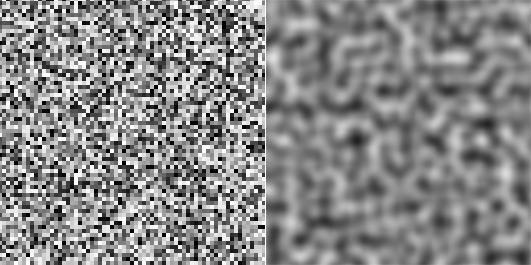
\includegraphics[width=0.8\linewidth]{img/noise-whitenoise.png}
    \caption{Diferença entre \textit{Value Noise} (à esquerda) e \textit{Perlin Noise} (à direita).}
    \label{fig:whitenoise}
\end{figure}

Em um espaço vetorial de coordenadas inteiras $[x, y, z]$, uma função hash $H()$ é utilizada para mapear cada coordenada a um valor pseudo-aleatório. Essa função é essencial para a reprodutibilidade do ruído.

Uma vez que o valor de ruído $Noise([x, y, z])$ é calculado, ele pode ser interpretado como um sinal para a modulação de cores, posições ou outras propriedades de um objeto. A aplicação do ruído pode gerar perturbações em texturas, como visto nas Figuras \ref{fig:donut_noise}, \ref{fig:sphere_noise} e \ref{fig:cube_noise}.

\begin{figure}[H]
    \centering
    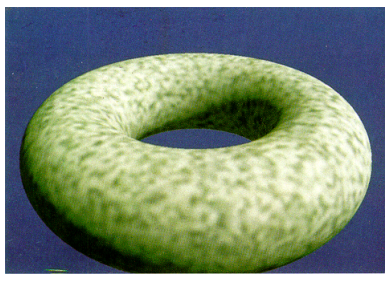
\includegraphics[width=0.4\textwidth]{img/donut.png}
    \caption{Donut com textura Noise aplicada}
    \label{fig:donut_noise}
\end{figure}

\begin{figure}[H]
    \centering
    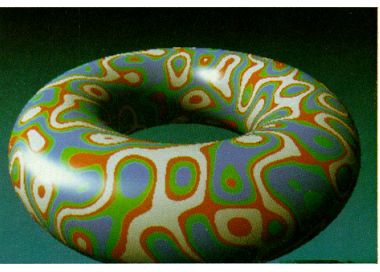
\includegraphics[width=0.4\textwidth]{img/donut2.png}
    \caption{Donut com textura Noise aplicada}
    \label{fig:sphere_noise}
\end{figure}

\begin{figure}[H]
    \centering
    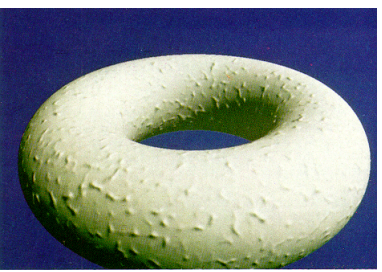
\includegraphics[width=0.4\textwidth]{img/donut3.png}
    \caption{Donut com textura Noise aplicada}
    \label{fig:cube_noise}
\end{figure}

A derivada do Perlin Noise, chamada de Dnoise(), é o vetor diferencial do ruído e representa a taxa de variação instantânea do ruído em cada uma das três direções do espaço. A aplicação do Dnoise() permite a criação de perturbações de superfície, influenciando, por exemplo, a normal de um objeto para simular relevo e detalhes finos.

$$
\text{normal} += \text{Dnoise}(\text{array})
$$

\begin{figure}[H]
    \centering
    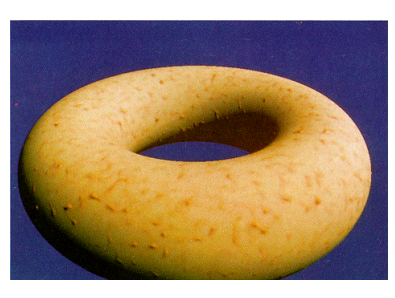
\includegraphics[width=0.4\textwidth]{img/donut4.png}
    \caption{Donut com textura Dnoise aplicada}
    \label{fig:donut_dnoise}
\end{figure}

Como estes cálculos são aplicados a nível de pixel em \textit{shaders}, a taxa de amostragem é fundamental. Frequências mais altas que a frequência de amostragem podem causar aliasing, um efeito indesejado. Para mitigar isso, as amostras são feitas de modo que a frequência do ruído se mantenha apropriada para a resolução do pixel.

O autor descreve uma técnica para simular a aparência de mármore usando a função \texttt{Noise()}. O método parte do princípio de que a aparência do mármore resulta de camadas heterogêneas que foram deformadas por forças turbulentas antes de se solidificarem. A abordagem é, portanto, uma combinação de uma estrutura regular e simples (as camadas) com uma complexa estrutura estocástica (o ruído da turbulência). A base do modelo são as camadas, representadas por uma simples onda senoidal, \texttt{sin(x)}. O autor usa a coordenada \texttt{point[1]} como o input para essa função, e o valor resultante é então mapeado para cores através de uma função auxiliar \texttt{marble\_color()}. Para adicionar o realismo das forças turbulentas, o autor introduz uma função \texttt{turbulence()}. Esta função é usada para perturbar a coordenada de entrada \texttt{x} antes que ela seja passada para a onda senoidal. O pseudocódigo que combina esses elementos é o seguinte:

\begin{lstlisting}[language=Python, caption={Pseudocódigo da função marble()}]
def marble(point):
  x = point[1] + turbulence(point)
  return marble_color(sin(x))
\end{lstlisting}

A função \texttt{turbulence()} é, por sua vez, uma soma de ruído em diferentes escalas, um processo que cria um padrão auto-semelhante ou \textit{1/f}. O algoritmo para a \texttt{turbulence()} é detalhado como:

\begin{lstlisting}[language=Python, caption={Pseudocódigo da função turbulence()}]
def turbulence(p):
  t = 0
  scale = 1
  while (scale > pixelsize):
    t += abs(Noise(p / scale) * scale)
    scale *= 2
  return t
\end{lstlisting}

Este procedimento garante que a quantidade de ruído adicionada em cada escala seja proporcional ao seu tamanho, resultando na impressão visual de movimento browniano. Além disso, o uso da função \texttt{abs()} em cada iteração assegura que o gradiente da textura tenha limites descontínuos em todas as escalas, o que é interpretado visualmente como fluxo turbulento.

\begin{figure}[H]
    \centering
    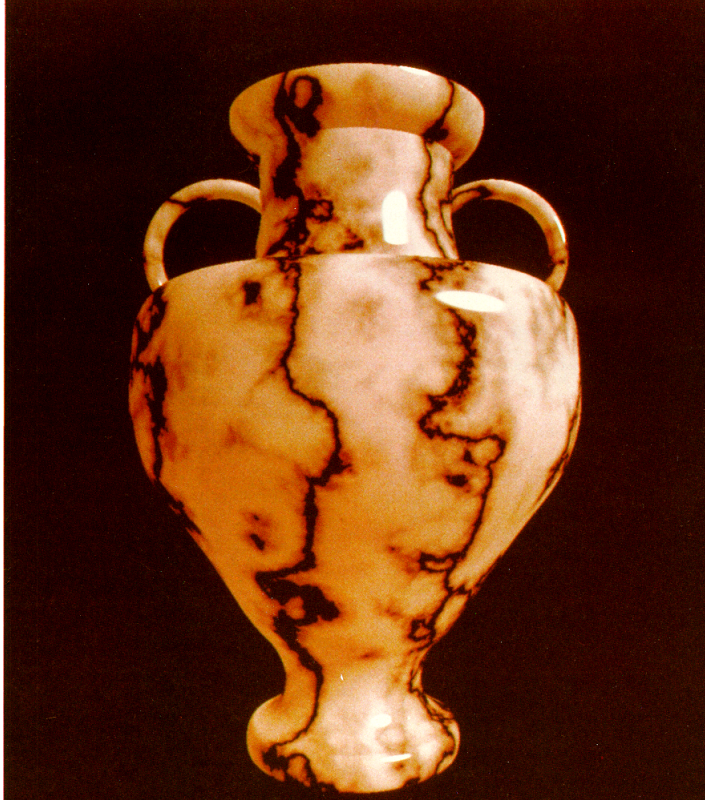
\includegraphics[width=0.4\textwidth]{img/marble.png}
    \caption{Textura de mármore gerada com a função marble()}
    \label{fig:marble_texture}
\end{figure}


\subsubsection{Mapeamento de Texturas Sólidas}
Qualquer função que mapeie um domínio de dimensões espaciais (como $\mathbb{R}^3$) para um valor (cor, por exemplo) pode ser considerada uma "função espacial". A partir disso, cada função espacial pode ser interpretada como a representação de um material sólido.

Desta forma, ao avaliar estas funções nos pontos visíveis da superfície de um objeto, é possível obter a textura da superfície, de modo parecido a ter "contornado" o objeto com o material. A textura obtida a partir deste tipo de extração é frequentemente tratada como uma textura sólida. Este termo é usado para descrever a representação de materiais que preenchem um volume, em vez de estarem apenas na superfície \cite{fractalNoise}.

\subsection{Ruído Fractal ou \textit{Fractional Browmian Motion} (fBm)}

A base para a geração procedural de terrenos é a criação de um mapa de alturas (\textit{heightmap}), onde o valor de brilho de um pixel corresponde à altitude de um ponto em um terreno. Um único ruído coerente, como o Perlin, gera um relevo excessivamente suave, como colinas perfeitamente arredondadas. Para criar a complexidade e os detalhes em múltiplas escalas de uma paisagem natural, o Ruído Fractal é aplicado.

A técnica consiste em somar várias camadas de ruído (chamadas de \textbf{oitavas}), cada uma contribuindo com um nível diferente de detalhe para a altitude final do terreno.

\begin{equation*}
\text{Altitude}(x, z) = \sum_{i=0}^{n-1} \text{amplitude}_i \cdot \text{Ruído}(\text{frequência}_i \cdot (x, z))
\end{equation*}

Os parâmetros que controlam a aparência do terreno são:
\begin{itemize}
\item \textbf{Oitavas (n):} O número de camadas de detalhe. As primeiras oitavas definem as cordilheiras principais e os vales. As últimas oitavas adicionam a rugosidade da superfície, como rochas e solo irregular.
\item \textbf{Lacunaridade (L):} Controla o aumento da frequência a cada oitava (tipicamente 2.0). Em termos práticos, define quão rapidamente os detalhes ficam menores. Uma lacunaridade alta cria terrenos com uma transição brusca entre as feições grandes e a rugosidade fina.

\item \textbf{Persistência (P):} Controla a diminuição da amplitude a cada oitava (tipicamente 0.5). Este é o parâmetro mais importante para o "sentimento" do terreno. Uma persistência baixa ($<0.5$) cria terrenos mais suaves e erodidos, onde as formas principais dominam. Uma persistência alta ($>0.5$) resulta em terrenos mais caóticos e rochosos, com grande influência dos detalhes finos.

\end{itemize}

\subsubsection{Criando Terrenos Rochosos com Ruído Turbulento}
Para modelar terrenos com características mais abruptas, como montanhas escarpadas ou cânions, uma variação chamada \textbf{Turbulência} é utilizada. Em vez de somar o ruído diretamente, somamos seu valor absoluto.
\begin{equation*}
\text{Altitude}{\text{turbulenta}}(x, z) = \sum{i=0}^{n-1} \text{amplitude}_i \cdot |\text{Ruído}(\text{frequência}_i \cdot (x, z))|
\end{equation*}
Esta simples modificação transforma os vales suaves em cumes afiados e ravinas, conferindo um aspecto mais "quebrado" e agressivo à paisagem, ideal para terrenos rochosos e vulcânicos.

\subsubsection{Simulando Erosão e Feições Orgânicas com Distorção de Domínio}
Para criar paisagens mais realistas e orgânicas, como vales de rios sinuosos ou padrões de erosão, a técnica de \textbf{Distorção de Domínio} (\textit{Domain Warping}) é aplicada. A ideia é usar uma função de ruído para "deformar" as coordenadas de entrada de outra.

Por exemplo, a altitude de um ponto (x,z) não é calculada diretamente. Primeiro, calculamos um deslocamento usando outro ruído:
\begin{align*}
    \text{deslocamento}_x &= C \cdot \text{fBm}_1(x, z) \\
    \text{deslocamento}_z &= C \cdot \text{fBm}_2(x, z)
\end{align*}
E então usamos as coordenadas distorcidas para calcular a altitude final:
\begin{equation*}
\text{Altitude}(x, z) = \text{fBm}{\text{base}}(x + \text{deslocamento}_x, z + \text{deslocamento}_z)
\end{equation*}
O resultado são terrenos com feições que parecem fluir e se conectar de maneira natural, simulando o efeito de forças como água e vento esculpindo a paisagem ao longo do tempo.

\subsection{O Algoritmo Diamond-Square}

Enquanto o Ruído Fractal (fBm) constrói um terreno somando ruídos em diferentes escalas (uma abordagem \textit{bottom-up}), o algoritmo \textbf{Diamond-Square} gera terrenos fractais através de um processo de subdivisão recursiva (uma abordagem \textit{top-down}). Ele opera sobre um grid quadrado cujas dimensões devem ser uma potência de dois mais um (ex: $2^n + 1$).

O algoritmo é inicializado com valores de altitude nos quatro cantos do grid e, em seguida, itera através de dois passos principais até que todo o grid seja preenchido:

\begin{enumerate}
    \item \textbf{Passo Diamante (Diamond Step):} Para cada quadrado no grid, o ponto central (o "diamante") recebe um valor de altitude que é a média dos quatro cantos do quadrado, acrescido de um pequeno deslocamento aleatório.

    \item \textbf{Passo Quadrado (Square Step):} Para cada diamante recém-criado, o ponto central de cada uma das suas quatro arestas (formando um "quadrado" rotacionado) recebe um valor de altitude. Esse valor é a média dos pontos vizinhos do diamante, acrescido de um deslocamento aleatório. Para os pontos nas bordas do grid, a média é calculada com apenas três pontos vizinhos.

    \item \textbf{Recorrência:} A cada iteração, a magnitude do deslocamento aleatório é reduzida. O processo é repetido para os novos quadrados menores que foram formados, até que todos os pontos do grid tenham um valor de altitude.
\end{enumerate}

O Diamond-Square é um método clássico, rápido e relativamente simples de implementar. No entanto, sua principal desvantagem é a tendência a gerar artefatos visuais, como cumes e vales alinhados com os eixos X e Y do grid, algo que o Perlin Noise evita naturalmente.

\subsection{Pós-Processamento e Realismo através da Simulação de Erosão Hidráulica}

Os terrenos gerados por algoritmos puramente matemáticos, como o fBm ou o Diamond-Square, muitas vezes carecem do realismo forjado por milênios de forças naturais. Para preencher essa lacuna, aplicamos algoritmos de simulação física como um passo de pós-processamento, sendo a erosão hidráulica um dos mais impactantes.

Essa técnica simula o efeito da água escoando sobre a superfície do terreno, esculpindo-o de forma natural. Um modelo comum é baseado na simulação de partículas (gotículas de chuva):

\begin{itemize}
    \item \textbf{Criação:} Milhares de "gotas d'água" são simuladas, cada uma sendo posicionada em um ponto aleatório do terreno.

    \item \textbf{Escoamento:} A gota calcula o gradiente de altitude ao seu redor e move-se para o vizinho mais baixo, simulando o fluxo da água morro abaixo.

    \item \textbf{Erosão:} À medida que a gota se move e ganha velocidade, ela "erode" uma pequena quantidade de sedimento do terreno, diminuindo a altitude dos pontos por onde passa.

    \item \textbf{Transporte e Deposição:} A gota carrega o sedimento consigo. Quando sua velocidade diminui (por exemplo, ao atingir uma área mais plana), ela perde a capacidade de carregar o material e o "deposita", aumentando a altitude do terreno naquele local.

    \item \textbf{Evaporação:} Após um certo tempo ou distância percorrida, a gota "evapora", e o ciclo recomeça com uma nova gota.
\end{itemize}

O resultado final é um terreno muito mais convincente, com a formação de redes de rios, vales suavizados, ravinas íngremes e planícies de aluvião, características que são extremamente difíceis de gerar apenas com funções de ruído \cite{erosion}.


\section{Simulação de Fluidos em Computação Gráfica}

Os maiores desafios da simulação de fluidos está nos aspectos fisicos que se aplicam, como por exemplo, convecção, difusão, turbulência e tensão superficial \cite{desbrun1996}. No entanto, essas simulações eram (ao menos em 2003) quase inviáveis para serem empregadas em tempo real, portanto a precisão acaba sendo deixada parcialmente de lado nestas simulações.

A simulação de fluidos começou, basicamente, com a equação de de Navier-Stokes (que será abordada na seção \ref{sec:volumes}) que descrevem a dinamica dos fluidos (esse sistema de equações diferenciais se baseia em derivadas parciais e permitem determinar os campos de velocidade e de pressão num escoamento de fluidos). 

\subsection{Smoothed Particle Hydrodynamics}

Em 1983, T. Reeves \cite{reeves1983} introduziu sistemas de partículas como uma técnica para modelar uma classe de objetos difusos. Desde então, tanto a abordagem Lagrangiana baseada em partículas quanto a abordagem Euleriana baseada em grades têm sido usadas para simular fluidos em computação gráfica. Desbrun e Cani \cite{desbrun1996} e Tonnesen \cite{tonnesen1998} utilizam partículas para animar objetos macios. As partículas também foram usadas para animar superfícies \cite{witkin1991}, controlar superfícies implícitas \cite{bloomenthal1997} e animar fluxos de lava \cite{carlson2002}. Nos últimos anos, a abordagem Euleriana tem sido mais popular para a simulação de fluidos em geral \cite{fedkiw2001}, água \cite{stam1999, foster1996, enright2002}, objetos macios \cite{muller2002} e efeitos de derretimento \cite{carlson2002}.

Em consonância, o artigo de Müller et al. (2003) \cite{muller2003} apresenta uma abordagem eficiente para simulação de fluidos baseada em Smoothed Particle Hydrodynamics (SPH). O método SPH representa o fluido como um conjunto de partículas, onde cada partícula carrega propriedades como massa, posição, velocidade e densidade. As interações entre partículas são calculadas usando funções de suavização (kernels), permitindo simular efeitos como pressão, viscosidade e forças externas.

As principais fórmulas utilizadas no SPH são:

\begin{itemize}
  \item Densidade: $$
\rho_i = \sum_j m_j W(|\mathbf{r}_i - \mathbf{r}_j|, h)
$$
onde $\rho_i$ é a densidade da partícula $i$, $m_j$ é a massa da partícula $j$, $W$ é o kernel de suavização e $h$ é o raio de influência.

\item Pressão: $$
\mathbf{f}_i^{\text{pressão}} = -\sum_j m_j \frac{p_i + p_j}{2 \rho_j} \nabla W(|\mathbf{r}_i - \mathbf{r}_j|, h)
$$
onde $p_i$ e $p_j$ são as pressões das partículas $i$ e $j$.

\item Viscosidade: $$
\mathbf{f}_i^{\text{visc}} = \mu \sum_j m_j \frac{\mathbf{v}_j - \mathbf{v}_i}{\rho_j} \nabla^2 W(|\mathbf{r}_i - \mathbf{r}_j|, h) $$ onde $\mu$ é o coeficiente de viscosidade e $\mathbf{v}_i$, $\mathbf{v}_j$ são as velocidades das partículas.
\end{itemize}

Essas fórmulas permitem calcular as forças que atuam sobre cada partícula, resultando em simulações de líquidos realistas e eficientes para aplicações interativas. Há de se notar, entretanto, que essas fórmulas tendem a ser muito custosas se implementadas conforme a descrição, sem otimização linear inclusa. Logo, diversos papers foram publicados visando manter qualidade suficiente, mas reduzindo o custo computacional e permitindo que essa simulação seja feita em tempo real. 


\subsection{Nuvens Volumétricas}
\label{sec:volumes}

Ao simular um fluído em tempo real, tem-se o desafio de preservar a performance computacional, sem perder muita qualidade visual. Para isso, técnicas de simulação Eulerianas baseadas em grades são frequentemente utilizadas,  onde o espaço é dividido em células (voxels) e as propriedades do fluído, como densidade, velocidade e pressão, são armazenadas em cada uma delas. Essas propriedades são então atualizadas ao longo do tempo usando métodos numéricos que resolvem as equações de Navier-Stokes, que governam o comportamento dos fluidos. Os volumes serão abordados aqui de 2 formas, modelagem de forma e shading, de maneira a se melhor representar materiais como fumaça, fogo, água, poeira, folhas, etc.

\subsubsection{Modelagem de forma}
No geral, ao se computar campos de particulas, espera-se que todas elas tenham seu tempo de vida bem definido para que se possa modelar de maneira precisa o seu comportamento. No entanto, em tempo real, esse trabalho se torna muito custoso. O movimento desses elementos passa a ser calculado, então, convertendo as velocidades que circulam o objeto em forças aplicadas sobre o corpo.

A poeira, por exemplo, pode ser modelada sendo carregada por um vetor de velocidades, sem que haja qualquer resistência significativa ou força externa a ser calculada. Entretanto, no caso da fumaça ou das nuvens, as particulas são substituidas pela simulação da densidade do fluido, que tenta aproximar a quantidade de particulas presentes no espaço (normalmente um valor entre 0 e 1). Essa descrição é dada pela função (conhecida como equação escalar de advecção-difusão):

$$
\frac{\partial \rho}{\partial t} = - (u \cdot \nabla) \rho + D \nabla^2 \rho + S
$$

Onde 
\begin{itemize}
  \item $\rho$ é a densidade de particulas, que varia no espaço e no tempo,
  \item $t$ é o tempo do sistema,
  \item $u$ é o campo de velocidades, ou seja, um vetor que indica a direção e a magnitude do movimento do fluido em cada ponto do espaço,
  \item $D$ é o coeficiente de difusão, que controla a taxa de dispersão das particulas no fluido (quanto maior o valor, mais rápido as particulas se espalham),
  \item $S$ é a fonte (ou sumidouro) de particulas,
  \item $\nabla$ é o operador nabla, que representa o gradiente espacial (uma medida de como a densidade muda no espaço),
  \item $\nabla^2$ é o operador laplaciano, que representa a difusão espacial (uma medida de como a densidade se espalha no espaço),
\end{itemize}

A \textbf{equação de advecção-difusão} pode ser resolvida numericamente alterando a grade supracitada, sendo sua resolução altamente importante para a precisão e o custo computacional da simulação, visto que grades mais finas proporcionam maior detalhe, mas exigem mais memória e poder de processamento. Segundo Stam et al \cite{Stam2003}, o método pode ser dividido em dois passos principais: o passo de densidade e o passo de velocidade, vistos a seguir.

\subsubsection*{Passo de Densidade}
O método linear (proposto por Stam at al \cite{Stam2003}) inicia-se com algum estado para as grades de velocidade e densidade e, então, atualiza seus valores baseado em eventos externos (forças, fonte de energia, fontes de particulas e etc.). Esse método se tornou famoso por ser estável para grandes passos de tempo (estabilidade incondicional) \footnote{Isso significa que, para qualquer valor positivo do passo de tempo, o método não produzirá resultados divergentes ou instáveis.}, o que é uma grande vantagem para simulações em tempo real. A cada passo de tempo, o método segue três etapas principais, passando pela equação de advecção-difusão de maneira "inversa", começando do termo final e indo para o inicial:

\begin{itemize}
  \item Primeiro termo (Source/Fonte): Adiciona densidade ao sistema baseado em fontes externas. Isso pode incluir a adição de fumaça de uma chaminé ou a introdução de calor em uma área específica.
  \item Segundo termo (Diffusion/Difusão): Simula a dispersão da densidade ao longo do tempo (se $D > 0$). Uma possível implementação é usar o método de Gauss-Seidel para resolver a equação de difusão, dada por 
    $$
    x_{k+1} = x_k + a \nabla^2 x_{k+1}
    $$
    onde $a$ é uma constante que depende do coeficiente de difusão e do passo de tempo. 

    Ou podemos usar o método de Jacobi, que é mais simples de implementar, mas pode ser menos eficiente. A equação de difusão usando o método de Jacobi é dada por:
    $$
    x_{k+1} = x_k + a \nabla^2 x_k
    $$

  \item Terceiro termo (Advection/Advecção): Podemos modelar o centro de cada célula da grade como se fosse uma particula que se move baseada na velocidade do campo. Assim, a densidade é transportada ao longo do campo de velocidades. Entretanto, temos que converter novamente as particulas para a celula proveniente. Uma maneira de fazer isso é usando o método de traçado de linha (backtrace), onde cada célula da grade é atualizada com a densidade da célula de onde a particula veio, baseado na velocidade do campo, ou seja, nos tracamos a linha de volta. Esse método é conhecido como "semi-Lagrangian advection" e é estável para grandes passos de tempo.

\end{itemize}

Temos como entrada na função o tamanho da matriz (N), a matriz de densidade atual (x), a matriz de densidade anterior (x0), as matrizes de velocidade (u e v), o coeficiente de difusão (diff) e o passo de tempo (dt). A função começa adicionando fontes de densidade, depois difunde a densidade e finalmente a advecta ao longo do campo de velocidades.

Percebe-se que, neste caso, temos 2 campos de velocidade (u e v), o que indica que estamos trabalhando em 2D. Para 3D, teríamos um terceiro campo de velocidade (w) e a função de advecção precisaria ser ajustada para levar isso em conta.

O codigo no final se aproxima disso:
\begin{lstlisting}[language=C]
void dens_step(int N, float *x, float *x0, 
float *u, float *v, float diff, float dt) {
  add_source (N, x, x0, dt);
  SWAP(x0, x); diffuse (N, 0, x, x0, diff, dt);
  SWAP(x0, x); advect (N, 0, x, x0, u, v, dt);
}
\end{lstlisting}


\subsubsection*{Passo de Velocidade}
O passo de velocidade é similar ao passo de densidade, mas com algumas diferenças importantes. Podemos dizer que a velocidade do campo se altera de 3 maneiras distintas: forças externas, difusão e advecção própria (ou auto-advecção - no qual o campo move a si mesmo). De maneira geral, pode ser descrito pela seguinte equação:

$$\frac{\partial u}{\partial t} = - (u \cdot \nabla) u + \nu \nabla^2 u + f - \frac{1}{\rho} \nabla p$$

Onde:
\begin{itemize}
  \item $u$ é o campo de velocidades,
  \item $t$ é o tempo do sistema,
  \item $\nu$ é o coeficiente de viscosidade (definido pelo usuário),
  \item $f$ é a força externa aplicada ao campo de velocidades,
  \item $(u \cdot \nabla)$ é o operador de advecção, que representa o transporte do campo de velocidades por ele mesmo,
  \item $\nabla^2$ é o operador laplaciano, que representa a difusão espacial do campo de velocidades.
  \item $\frac{1}{\rho} \nabla p$ é o termo de pressão, que representa a força devido à variação de pressão no fluido.
\end{itemize}

O código desta etapa pode ser escrito como:

\begin{lstlisting}[language=C]
void vel_step(int N, fl oat *u, float *v, 
float *u0, float *v0, float visc, float dt) {
  add_source(N, u, u0, dt); add_source(N, v, v0, dt);
  SWAP(u0, u); diffuse(N, 1, u, u0, visc, dt);
  SWAP(v0, v); diffuse(N, 2, v, v0, visc, dt);
  project(N, u, v, u0, v0);
  SWAP(u0, u); SWAP( v0, v);
  advect(N, 1, u, u0, u0, v0, dt);
  advect(N, 2, v, v0, u0, v0, dt);
  project(N, u, v, u0, v0);
}
\end{lstlisting}

Note que temos um novo procedimento neste passo chamado \texttt{project}, que é responsável por garantir que o campo de velocidades seja incompressível, ou seja, que a divergência do campo seja zero ($\nabla \cdot u = 0$) \footnote{a massa do fluido permanece constante ao longo do tempo.}. Isso é importante para simular fluidos realistas, onde a massa é conservada. Este método pode ser implementado resolvendo a equação de Poisson para o componente de pressão e, em seguida, ajustando o campo de velocidades com base no gradiente resultante.

O procedimento \texttt{project} calcula a pressão p que seria necessária para "empurrar" o excesso de massa para fora (ou puxar a falta de massa para dentro) e, em seguida, aplica a força de pressão ($-\nabla p$) para corrigir as velocidades e pode ser implementado da seguinte maneira:

\begin{lstlisting}[language=C]
void project(int N, float *u, float *v, float *p, float *div) {
  int i, j, k;
  float h = 1.0f / N;
  for (i = 1; i <= N; i++) {
    for (j = 1; j <= N; j++) {
      div[IX(i,j)] = -0.5f*h*(u[IX(i+1,j)]
      - u[IX(i-1,j)] + v[IX(i,j+1)] - v[IX(i,j-1)]);
      p[IX(i,j)] = 0;
    }
  }
  set_boundary(N, 0, div); set_boundary(N, 0, p);

  for (k = 0; k < 20; k++) {
    for (i = 1; i <= N; i++) {
      for (j = 1; j <= N; j++) {
        p[IX(i,j)] = (div[IX(i,j)] + p[IX(i-1,j)]
        + p[IX(i+1,j)] + p[IX(i,j-1)] + p[IX(i,j+1)]) / 4;
      }
    }
    set_boundary(N, 0, p);
  }

  for (i = 1; i <= N; i++) {
    for (j = 1; j <= N; j++) {
      u[IX(i,j)] -= 0.5f*(p[IX(i+1,j)] - p[IX(i-1,j)])/h;
      v[IX(i,j)] -= 0.5f*(p[IX(i,j+1)] - p[IX(i,j-1)])/h;
    }
  }
  set_boundary(N, 1, u); set_boundary(N, 2, v);
}
\end{lstlisting}

\subsubsection{Conclusão da modelagem de forma}
Podemos concluir essa seção com a presença de uma rotina principal, que chama os passos de densidade e velocidade, atualizando o estado do fluido a cada frame \footnote{A rotina \texttt{draw\_dens} será abordada na seção de shading \ref{sec:shading}.};. 
\begin{lstlisting}[language=C]
void simulate(int N, float *u, float *v, float *u0, float *v0,
float *dens, float *dens0, float diff, float visc, float dt) {
  get_inputs(N, u0, v0, dens0);
  vel_step(N, u, v, u0, v0, visc, dt);
  dens_step(N, dens, dens0, u, v, diff, dt);
  draw_dens(N, dens);
}
\end{lstlisting}

\subsection{Shading}
\label{sec:shading}

Volumes são tradicionalmente renderizados usando soluções numéricas para a equação de rendering volumétrico, descrita a seguir:

$$
L(x_0, \omega) = \int_{0}^{t_{max}} (\sigma_s(X(t)) L_i(X(t), \omega) + L_e(X(t), \omega))e^{-\int_{0}^{t} \sigma_t(X(s)) ds} dt
$$

Onde
\begin{itemize}
  \item $L(x_0, \omega)$ é a radiância (cor) na posição $x_0$ na direção $\omega$,
  \item $t_{max}$ é a distância máxima que o raio percorre no volume,
  \item $X(t) = x_0 + t\omega$ é a posição ao longo do raio,
  \item $\sigma_s(X(t))$ é o coeficiente de espalhamento no ponto $X(t)$,
  \item $L_i(X(t), \omega)$ é a radiância incidente no ponto $X(t)$ na direção $\omega$,
  \item $L_e(X(t), \omega)$ é a radiância emitida no ponto $X(t)$ na direção $\omega$,
  \item $\sigma_t(X(s)) = \sigma_a(X(s)) + \sigma_s(X(s))$ é o coeficiente de atenuação total no ponto $X(s)$, que é a soma dos coeficientes de absorção ($\sigma_a$) e espalhamento ($\sigma_s$),
  \item $e^{-\int_{0}^{t} \sigma_t(X(s)) ds}$ é o termo de atenuação, que representa a redução da radiância devido à absorção e espalhamento ao longo do caminho do raio.
\end{itemize}

Uma abordagem comum é o método de \textbf{\textit{ray marching}}, onde um raio é lançado através do volume e amostras são coletadas ao longo do caminho do raio. Essas amostras são então usadas para calcular a cor e a opacidade do pixel correspondente na imagem final.

\subsubsection{Interação da luz com volumes}

Vamos tratar dos fenomenos físicos descritos pela equação de rendering volumétrico, passando por absorção, emissão e espalhamento e como eles podem ser implementados em um sistema de ray marching.

\begin{itemize}
  \item Absorção: A luz é absorvida pelo meio, reduzindo sua intensidade. Isso é descrito pela lei de Beer-Lambert:
  $$
  I(t) = I_0 e^{-\int_{0}^{t} \sigma_a(s) ds}
  $$
  onde $I(t)$ é a intensidade da luz no ponto $t$, $I_0$ é a intensidade inicial, e $\sigma_a(s)$ é o coeficiente de absorção no ponto $s$.
  
  \item Emissão: O meio pode emitir luz, contribuindo para a intensidade total. A contribuição da emissão pode ser modelada como:
  $$
  L_{emit}(t) = \int_{0}^{t} j(s) e^{-\int_{s}^{t} \sigma_a(u) du} ds
  $$
  onde $j(s)$ é a taxa de emissão no ponto $s$.
  
  \item Espalhamento: A luz pode ser espalhada em diferentes direções ao interagir com o meio. O espalhamento pode ser descrito pela função de fase $p(\omega', \omega)$, que define a probabilidade de um raio de luz ser espalhado da direção $\omega'$ para a direção $\omega$. A contribuição do espalhamento pode ser modelada como:
  $$
  L_{scatter}(t) = \int_{0}^{t} \sigma_s(s) \int_{S^2} p(\omega', \omega) L(s, \omega') d\omega' e^{-\int_{s}^{t} \sigma_a(u) du} ds
  $$
  onde $\sigma_s(s)$ é o coeficiente de espalhamento no ponto $s$, e $L(s, \omega')$ é a radiância incidente na direção $\omega'$ no ponto $s$ \cite{Kajiya1984}.
\end{itemize}

Todas essas técnicas se acumulam na equação de rendering volumétrico expressa no inicio da seção \ref{sec:shading}. A implementação das técnicas de solução numérica pode variar dependendo do contexto específico e dos requisitos de desempenho e qualidade visual, mas o objetivo geral é capturar a complexidade da interação da luz com volumes de maneira eficiente e realista, mantendo a precisão física e sem fritar o seu chip gráfico.

\subsubsection{Implementação básica de ray marching}
Trataremos agora de uma implementação básica de ray marching para volumes, que incorpora os conceitos de absorção, emissão e espalhamento discutidos anteriormente. 
Essa implementação envolve o lançamento de um raio através do volume e a amostragem da densidade e outras propriedades do volume ao longo do caminho do raio. O código a seguir ilustra uma implementação do comportamento esperado:

\begin{lstlisting}[language=C]
vec4 ray_march(vec3 ray_origin, vec3 ray_direction,
float t_near, float t_far) {
  vec4 color = vec4(0.0);
  float t = t_near;
  float step_size = 0.1;
  while (t < t_far) {
    vec3 sample_position = ray_origin + t * ray_direction;
    float density = sample_density(sample_position);
    vec4 sample_color = compute_color(density);
    color += sample_color * exp(-density * step_size);
    t += step_size;
  }
  return color;
}
\end{lstlisting}

Este código define uma função `ray\_march` que toma a origem e a direção do raio, bem como os limites próximo e distante do volume. A função itera ao longo do caminho do raio, amostrando a densidade do volume em cada passo e acumulando a cor resultante, levando em consideração a absorção da luz. A função `sample\_density` é responsável por retornar a densidade do volume em uma posição específica, enquanto a função `compute\_color` calcula a cor com base na densidade amostrada. A variável `step\_size` controla a distância entre as amostras ao longo do raio, e pode ser ajustada para equilibrar a qualidade visual e o desempenho. Note que esta é uma implementação simplificada e pode ser expandida para incluir efeitos adicionais, como emissão e espalhamento, conforme discutido anteriormente \cite{Pharr2016}.
\section{Volumes (baseado em particulas)}
\label{sec:volumes}

Volumes em geral podem ser descritos de diversas maneiras, dentre elas, campos de particulas, campos de voxels, SDFs, entre outros. Os volumes serão abordados aqui de 2 formas, modelagem de forma e shading, de maneira a se melhor representar volumes como fumaça, fogo, agua, poeira, folhas, etc.

\subsection{Modelagem de forma}
No geral, ao se computar campos de particulas, espera-se que todas elas tenham seu \textit{lifetime} bem definido para que se possa modelar de maneira precisa o seu comportamento. No entanto, em tempo real, esse trabalho se torna muito custoso, especialmente para volumes que representam fumaca ou folhas ou ate mesmo agua. O movimento desses elementos passa a ser calculado, entao, convertendo as velocidades que circulam o objeto em forcas de corpo. Vemos que poeira simplesmente pode ser modelada sendo carregada pelo vetor de velocidades, sem qualquer resistência significativa. Entretanto, no caso da fumaça, as particulas são substituidas por uma densidade de particulas que aproximam a quantidade delas presentes (normalmente um valor entre 0 e 1). Essa descrição é dada por essa função (conhecida como equação de advecção-difusão): 

$$
\frac{\partial \rho}{\partial t} = - (u \cdot \nabla) \rho + D \nabla^2 \rho + S
$$

Onde $u$ é o campo de velocidades, $D$ é o coeficiente de difusão e $S$ é a fonte de particulas. A equação de advecção-difusão pode ser resolvida numericamente usando métodos como diferenças finitas ou volumes finitos. Esses métodos envolvem a discretização do domínio em uma grade e a atualização dos valores da densidade em cada célula da grade ao longo do tempo com base na equação diferencial parcial \cite{Stam2003}.

Esse cálculo normalmente é atribuido a um grid (matriz) bidimensional ou tridimensional, onde cada célula da grade armazena informações sobre a densidade de particulas, velocidade e outras propriedades relevantes. A resolução da grade afeta diretamente a precisão e o custo computacional da simulação. Grades mais finas proporcionam maior detalhe, mas exigem mais memória e poder de processamento.

\subsubsection{Passo de Densidade}
O método linear proposto por Stam at al \cite{Stam2003} inicia-se com algum estado para a velocidade e densidade e, então, atualiza seus valores baseado em eventos externos (forças, fonte de energia, fontes de particulas e etc.). A cada passo de tempo, o método segue três etapas principais, passando pela equação de advecção-difusão de maneira "inversa", começando do termo final e indo para o inicial:

\begin{itemize}
  \item Primeiro termo (Source/Fonte): Adiciona densidade ao sistema baseado em fontes externas. Isso pode incluir a adição de fumaça de uma chaminé ou a introdução de calor em uma área específica.
  \item Segundo termo (Diffusion/Difusão): Simula a dispersão da densidade ao longo do tempo (se $D > 0$). Uma possível implementação é usar o método de Gauss-Seidel para resolver a equação de difusão, dada por 
    $$
    x_{k+1} = x_k + a \nabla^2 x_{k+1}
    $$
    onde $a$ é uma constante que depende do coeficiente de difusão e do passo de tempo.
  \item Terceiro termo (Advection/Advecção): Podemos modelar o centro de cada célula da grade como se fosse uma particula que se move baseada na velocidade do campo. Assim, a densidade é transportada ao longo do campo de velocidades. Entretanto, temos que converter novamente as particulas para a celula proveniente. Uma maneira de fazer isso é usando o método de traçado de linha (backtrace), onde cada célula da grade é atualizada com a densidade da célula de onde a particula veio, baseado na velocidade do campo, ou seja, nos tracamos a linha de volta. Esse método é conhecido como "semi-Lagrangian advection" e é estável para grandes passos de tempo.

\end{itemize}

O codigo no final vai ter essa cara:
\begin{lstlisting}[language=C]
void dens_step(int N, float *x, float *x0, 
float *u, float *v, float diff, float dt) {
  add_source (N, x, x0, dt);
  SWAP(x0, x); diffuse (N, 0, x, x0, diff, dt);
  SWAP(x0, x); advect (N, 0, x, x0, u, v, dt);
}
\end{lstlisting}

\subsubsection{Passo de Velocidade}
O passo de velocidade é similar ao passo de densidade, mas com algumas diferenças importantes. Podemos dizer que a velocidade do campo se altera de 3 maneiras distintas: forças externas, difusão e advecção própria (ou auto-advecção - no qual o campo move a si mesmo). O código desta etapa pode ser escrito como:

\begin{lstlisting}[language=C]
void vel_step(int N, fl oat *u, float *v, 
float *u0, float *v0, float visc, float dt) {
  add_source(N, u, u0, dt); add_source(N, v, v0, dt);
  SWAP(u0, u); diffuse(N, 1, u, u0, visc, dt);
  SWAP(v0, v); diffuse(N, 2, v, v0, visc, dt);
  project(N, u, v, u0, v0);
  SWAP(u0, u); SWAP( v0, v);
  advect(N, 1, u, u0, u0, v0, dt);
  advect(N, 2, v, v0, u0, v0, dt);
  project(N, u, v, u0, v0);
}
\end{lstlisting}

Note que temos um novo procedimento neste passo chamado \texttt{project}, que é responsável por garantir que o campo de velocidades seja incompressível, ou seja, que a divergência do campo seja zero. Isso é importante para simular fluidos realistas, onde a massa é conservada. Este método pode ser implementado resolvendo a equação de Poisson para a pressão e, em seguida, ajustando o campo de velocidades com base no gradiente da pressão.

O procedimento \texttt{project} pode ser implementado da seguinte maneira:
\begin{lstlisting}[language=C]
void project(int N, float *u, float *v, float *p, float *div) {
  int i, j, k;
  float h = 1.0f / N;
  for (i = 1; i <= N; i++) {
    for (j = 1; j <= N; j++) {
      div[IX(i,j)] = -0.5f*h*(u[IX(i+1,j)]
      - u[IX(i-1,j)] + v[IX(i,j+1)] - v[IX(i,j-1)]);
      p[IX(i,j)] = 0;
    }
  }
  set_boundary(N, 0, div); set_boundary(N, 0, p);

  for (k = 0; k < 20; k++) {
    for (i = 1; i <= N; i++) {
      for (j = 1; j <= N; j++) {
        p[IX(i,j)] = (div[IX(i,j)] + p[IX(i-1,j)]
        + p[IX(i+1,j)] + p[IX(i,j-1)] + p[IX(i,j+1)]) / 4;
      }
    }
    set_boundary(N, 0, p);
  }

  for (i = 1; i <= N; i++) {
    for (j = 1; j <= N; j++) {
      u[IX(i,j)] -= 0.5f*(p[IX(i+1,j)] - p[IX(i-1,j)])/h;
      v[IX(i,j)] -= 0.5f*(p[IX(i,j+1)] - p[IX(i,j-1)])/h;
    }
  }
  set_boundary(N, 1, u); set_boundary(N, 2, v);
}
\end{lstlisting}

\subsection{Conclusão da modelagem de forma}
Podemos concluir essa seção com esse código maravilhoso que junta tudo:

\begin{lstlisting}[language=C]
void simulate(int N, float *u, float *v, float *u0, float *v0,
float *dens, float *dens0, float diff, float visc, float dt) {
  get_inputs(N, u0, v0, dens0);
  vel_step(N, u, v, u0, v0, visc, dt);
  dens_step(N, dens, dens0, u, v, diff, dt);
  draw_dens(N, dens);
}
\end{lstlisting}

a rotina \texttt{draw\_dens} será abordada na seção de shading.

\subsection{Shading}
\label{sec:shading}

Volumes são tradicionalmente renderizados usando técnicas de ray marching, onde um raio é lançado através do volume e amostras são coletadas ao longo do caminho do raio. Essas amostras são então usadas para calcular a cor e a opacidade do pixel correspondente na imagem final. A equação de rendering para volumes pode ser expressa como:
$$
C = \int_{t_{near}}^{t_{far}} T(t) \sigma(t) L(t) dt
$$
onde $C$ é a cor final do pixel, $T(t)$ é a transmissão ao longo do caminho do raio, $\sigma(t)$ é a densidade de absorção no ponto $t$, e $L(t)$ é a luz incidente no ponto $t$. A transmissão $T(t)$ é dada por:
$$
T(t) = e^{-\int_{t_{near}}^{t} \sigma(s) ds}
$$

Existem diversas técnicas para otimizar o ray marching, como o uso de grids adaptativos, onde a resolução do grid é maior em áreas de interesse e menor em áreas menos importantes. Outra técnica é o uso de pré-computação de iluminação, onde a iluminação é calculada previamente e armazenada em uma textura 3D, que pode ser rapidamente acessada durante o ray marching. Além disso, técnicas de denoising podem ser aplicadas para reduzir o ruído nas imagens renderizadas, especialmente em simulações de volumes complexos como fumaça e fogo, no entanto, não serão abordadas aqui.

\subsubsection{Interação da luz com volumes}

A luz pode ser absorvida, emitida ou espalhada ao interagir com os volumes gerados até aqui, sendo cada um dos fenômenos descritos por uma equação específica:

\begin{itemize}
  \item Absorção: A luz é absorvida pelo meio, reduzindo sua intensidade. Isso é descrito pela lei de Beer-Lambert:
  $$
  I(t) = I_0 e^{-\int_{0}^{t} \sigma_a(s) ds}
  $$
  onde $I(t)$ é a intensidade da luz no ponto $t$, $I_0$ é a intensidade inicial, e $\sigma_a(s)$ é o coeficiente de absorção no ponto $s$.
  
  \item Emissão: O meio pode emitir luz, contribuindo para a intensidade total. A contribuição da emissão pode ser modelada como:
  $$
  L_{emit}(t) = \int_{0}^{t} j(s) e^{-\int_{s}^{t} \sigma_a(u) du} ds
  $$
  onde $j(s)$ é a taxa de emissão no ponto $s$.
  
  \item Espalhamento: A luz pode ser espalhada em diferentes direções ao interagir com o meio. O espalhamento pode ser descrito pela função de fase $p(\omega', \omega)$, que define a probabilidade de um raio de luz ser espalhado da direção $\omega'$ para a direção $\omega$. A contribuição do espalhamento pode ser modelada como:
  $$
  L_{scatter}(t) = \int_{0}^{t} \sigma_s(s) \int_{S^2} p(\omega', \omega) L(s, \omega') d\omega' e^{-\int_{s}^{t} \sigma_a(u) du} ds
  $$
  onde $\sigma_s(s)$ é o coeficiente de espalhamento no ponto $s$, e $L(s, \omega')$ é a radiância incidente na direção $\omega'$ no ponto $s$ \cite{Kajiya1984}.
\end{itemize}

Todas essas técnicas se acumulam na equação de rendering volumétrico expressa no inicio da seção \ref{sec:shading}, que pode ser resolvida numericamente usando métodos como ray marching ou path tracing. A implementação dessas técnicas pode variar dependendo do contexto específico e dos requisitos de desempenho e qualidade visual, mas o objetivo geral é capturar a complexidade da interação da luz com volumes de maneira eficiente e realista.

\subsubsection{Implementação básica de ray marching}
A implementação básica de ray marching envolve o lançamento de um raio através do volume e a amostragem da densidade e outras propriedades do volume ao longo do caminho do raio. O código a seguir ilustra uma implementação simples de ray marching para volumes:

\begin{lstlisting}[language=C]
vec4 ray_march(vec3 ray_origin, vec3 ray_direction,
float t_near, float t_far) {
  vec4 color = vec4(0.0);
  float t = t_near;
  float step_size = 0.1;
  while (t < t_far) {
    vec3 sample_position = ray_origin + t * ray_direction;
    float density = sample_density(sample_position);
    vec4 sample_color = compute_color(density);
    color += sample_color * exp(-density * step_size);
    t += step_size;
  }
  return color;
}
\end{lstlisting}

Este código define uma função `ray\_march` que toma a origem e a direção do raio, bem como os limites próximo e distante do volume. A função itera ao longo do caminho do raio, amostrando a densidade do volume em cada passo e acumulando a cor resultante, levando em consideração a absorção da luz. A função `sample\_density` é responsável por retornar a densidade do volume em uma posição específica, enquanto a função `compute\_color` calcula a cor com base na densidade amostrada. A variável `step\_size` controla a distância entre as amostras ao longo do raio, e pode ser ajustada para equilibrar a qualidade visual e o desempenho. Note que esta é uma implementação simplificada e pode ser expandida para incluir efeitos adicionais, como emissão e espalhamento, conforme discutido anteriormente \cite{Pharr2016}.

\section{Justificativa}
\label{sec:justificativa}
Justificativa

\subsection{Objetivos}

Este projeto tem, portanto, um foco educacional ao se utilizar uma ferramenta comum como o Unity e mostrar a viabilidade de se implementar uma simulação complexa e otimizada com GPU em tempo real, conduzindo uma experimentação de técnicas distinas, consonantemente a um aprimoramento academico dos alunos aqui presentes. Ao se desenvolver um sistema de geração volumétrica de nuvens em tempo real, esperamos alcançar os seguintes objetivos específicos:

\begin{itemize}
    \item \textbf{Implementação de técnicas de geração volumétrica:} Desenvolver e implementar técnicas avançadas de geração volumétrica de nuvens, como noise functions (Perlin, Simplex), Worley noise, e outras abordagens baseadas em shaders.
    \item \textbf{Otimização para tempo real:} Adaptar e otimizar os algoritmos de geração volumétrica para garantir que possam ser executados em tempo real dentro do Unity URP, mantendo um equilíbrio entre qualidade visual e desempenho.
    \item \textbf{Integração com Unity URP:} Integrar o sistema de geração volumétrica de nuvens com o Unity Universal Render Pipeline, aproveitando suas capacidades de renderização e iluminação para melhorar a aparência das nuvens.
\end{itemize}
\section{Metodologia}
\label{sec:metodologia}

A concretização dos objetivos educacionais deste projeto foi alcançada através da implementação de um sistema de simulação e renderização em tempo real, utilizando o motor Unity sob a arquitetura do \textit{Universal Render Pipeline} (URP). Esta plataforma foi selecionada por sua capacidade de integrar rotinas de computação aceleradas por GPU (GPGPU), um requisito fundamental para processar as simulações complexas em tempo real.

O \textit{pipeline} metodológico foi dividido em duas etapas principais, ambas executadas inteiramente no processador gráfico. A primeira etapa, a "modelagem de forma", consiste na simulação da dinâmica dos fluidos. Para este fim, foram empregados \textit{Compute Shaders} para resolver numericamente as equações que governam o comportamento dos fluidos, como a equação de advecção-difusão, que modela a densidade volumétrica. Esta abordagem permitiu a implementação eficiente dos passos de advecção (pelo método semi-Lagrangiano), difusão e adição de fontes, atualizando um \textit{grid} tridimensional que representa o estado do volume a cada quadro. Podemos ver a interação dos componentes do projeto no seguinte 'diagrama': 

\begin{figure}[H]
\label{fig:fluid_pipeline}
\centering
\begin{tikzpicture}[
    node distance=10mm and 18mm,  % Distância horizontal aumentada
    box/.style = {draw, rounded corners, minimum width=40mm, minimum height=10mm, align=center, font=\footnotesize, fill=blue!5},
    cloudstyle/.style = {draw, cloud, cloud puffs=12, cloud ignores aspect, minimum width=36mm, minimum height=18mm, align=center, font=\footnotesize, fill=gray!10},
    small/.style = {draw, rounded corners, minimum height=6mm, align=center, font=\scriptsize, fill=white},
    arr/.style = {->, >=Stealth, line width=0.7pt},
    faded/.style = {draw=black!50, text=black!70, fill=white, rounded corners, font=\scriptsize}
]

% --- Pipeline Principal ---
\node (cpu) [small] {CPU / Unity Engine};

\node (sim) [box, below=of cpu, node distance=14mm]
    {Etapa 1: Simulação de Fluidos \\ (Compute Shader)};

\node (data) [box, below=of sim, node distance=25mm, fill=green!10]
    {Grid 3D (Textura Volumétrica)};

\node (render) [box, below=of data, node distance=25mm]
    {Etapa 2: Renderização \\ (Volumetric Ray Marching)};

\node (output) [cloudstyle, below=of render, node distance=25mm]
    {Imagem Final (Nuvem Volumétrica)};

% --- Passos da Simulação) ---
\node (step_title) [font=\tiny\bfseries, left=of sim, node distance=45mm] {Passos da Simulação:};
\node (step1) [faded, below=of step_title, node distance=6mm] {Adição de Fontes};
\node (step2) [faded, below=of step1] {Difusão};
\node (step3) [faded, below=of step2] {Advecção (Semi-Lagrangiana)};

% Fluxo Principal
\draw [arr] (cpu) -- (sim)
    node [midway, right, font=\tiny, xshift=2mm] {Dispatch (GPU)};
\draw [arr, line width=1pt] (sim) -- (data)
    node [midway, right, font=\scriptsize, xshift=1mm] {Atualiza Grid (Write)};
\draw [arr, line width=1pt] (data) -- (render)
    node [midway, right, font=\scriptsize, xshift=1mm] {Amostra Grid (Read)};
\draw [arr] (render) -- (output);

\draw [arr, line width=1pt, dashed] (data.east) to [bend right=50] (sim.east)
    node [midway, right, font=\scriptsize, xshift=1mm] {};

\coordinate (sim_input) at (sim.west);
\draw [arr, dashed, faded] (step1.east) -- (sim_input);
\draw [arr, dashed, faded] (step2.east) -- (sim_input);
\draw [arr, dashed, faded] (step3.east) -- (sim_input);

\end{tikzpicture}
\caption{Diagrama do Pipeline de Simulação e Renderização de Fluidos Volumétricos}
\end{figure}


Subsequentemente, a segunda etapa consistiu na renderização deste volume dinâmico. Foi implementada a técnica de \textit{volumetric ray marching}, cuja fundamentação teórica foi apresentada na Seção 5. Um \textit{shader} customizado foi desenvolvido para marchar raios através do \textit{grid} de densidade, que é continuamente atualizado pelo \textit{Compute Shader}. Este \textit{shader} de renderização foi integrado ao URP para amostrar o volume e calcular a interação da luz (absorção e espalhamento), gerando a representação visual final das nuvens volumétricas.



\section{Resultados}
\label{sec:resultados}
Resultados

\section{Conclusão}
Concluido


\bibliographystyle{plain}
\bibliography{bibliography}
\end{document}
